\documentclass[11pt,makeidx,fleqn]{article}
\usepackage[intlimits,fleqn]{amsmath}
\usepackage{amssymb}
\usepackage{latexsym}
\usepackage{german}
%\usepackage{epsfig}
\usepackage{longtable}
\usepackage{array}
\ifx\pdfoutput\undefined
  \usepackage[xdvi]{epsfig}
\else
  \usepackage{graphicx}
\fi
%\documentstyle[amstex,style,11pt]{article}
\setlength{\parindent}{0mm}
\setlength{\textwidth}{140mm}
\setlength{\textheight}{240mm}
\setlength{\topmargin}{-1in}
\setlength{\headheight}{0in}
\setlength{\headsep}{1in}
%\setlength{\footheight}{0in}
\setlength{\footskip}{10mm}
\setlength{\oddsidemargin}{0.2in}
\setlength{\evensidemargin}{0.2in}
\setlength{\parskip}{4pt}                                                               

\renewcommand{\footnoterule}{\rule{\textwidth}{0.1ex} \vspace{-2ex}} 

\renewcommand{\footnotesize}{\scriptsize} 


\setcounter{secnumdepth}{5}   % bewirkt Aenderung der maximalen
                              % Kapitel-Nummerierung,
                              % hier von 3 (default) auf 5
\setcounter{tocdepth}{5}      % bewirkt Uebernahme der zusaetzlichen
                              % Kapitel-Ueberschriften ins Inhaltsverzeichnis
                                                                                              
%\usepackage{amsmath,amsthm,epsfig,amstext,amssymb,a4,makeidx,amscd,german}%amsfonts}
%\usepackage{graphicx,subfigure} %nickis Zeichnung??
%

\sloppy % fuer eine lockere Silbentrennung!!

\parindent0cm %keine Einrueckung nach Absatz
                
\pagestyle{myheadings} %kapitelueberschrift in Kopfzeile
\bibliographystyle{amsalpha}
%\DeclareGraphicsRule{.gif}{bmp}{}{}

\setlength{\doublerulesep}{0pt}                                                                              

\begin{document}

%***************************************************************************************

\newenvironment{list_sabina}{\begin{list}{$\bullet$}{\setlength{\labelwidth}{3mm} \setlength{\labelsep}{2mm} \setlength{\parsep}{1mm} \setlength{\topsep}{0mm} \setlength{\itemsep}{0mm}}}{\end{list}}
 
\newenvironment{sub_list_sabina}{\begin{list}{$\circ$}{\setlength{\labelwidth}{2.5mm} \setlength{\labelsep}{1mm} \setlength{\parsep}{1mm} \setlength{\topsep}{0mm} \setlength{\itemsep}{-1mm}}}{\end{list}}             

\newcommand{\myraise}[1]{\raisebox{-1.5ex}[0ex][-1.5ex]{#1}}


%***************************************************************************************


\pagestyle{empty}

\phantom{a}
\vspace{30mm}

\begin{center}
\underline{\underline{\Huge\bf Teil-Spezifikation}}\\[15mm]
{\Large\bf Multimediale}\\[2ex]
{\Large\bf Mathematikausbildung}\\[2ex]
{\Large\bf f"ur Ingenieure}\\[14ex]
{\Large\bf Navigationsframe}
\item \end{center}

\vspace{32mm}

\vspace{5mm}
\begin{center}
{\large \textbf{Autoren:}}\\[2.5ex] 
{\large Sabina Jeschke -- Erhard Zorn}
\end{center}


\vspace{10mm}

\begin{center}
{\large\bf Stand: Berlin, \today}
\end{center}

\begin{tabular}{ll}
\textsf{Datum:}&\verb+$Date: 2004/01/28 19:36:53 $+\\ % Wird vom cvs eingetragen
\textsf{CVS-Version:}&\verb+$Revision: 1.4 $+\\ % Wird vom cvs eingetragen
\textsf{CVS-Source:}&\verb+$Source: /net/mumie/cvs/styles/navigationframe/titel.tex,v $+\\ % Wird vom cvs eingetragen
\end{tabular}

\newpage

\phantom{was auch immer...}

\setcounter{page}{0}

\clearpage

\pagestyle{plain}

%**************************************************************************




\clearpage

\tableofcontents
\clearpage

\section{Skizzen zum ``Literarischen'' Style}\label{lit_style}

\begin{list_sabina}

\item
\textbf{Rechtschreibung:}\\
Es gelten die Regeln der \textit{neuen} Rechtschreibung.

\item
\textbf{Anglizismen:}\\
Anglizismen sind nach M"oglichkeit zu vermeiden.

\item
\textbf{Abk"urzungen:}\\
Abk"urzungen sind nach M"oglichkeit zu vermeiden.\\
Sie sind notfalls zul"assig, wenn sie der besseren "Ubersicht dienen
und in formelartigen Zusammenh"angen verwendet werden,
m"ussen dann aber im standalone-Sinne immer beim ihrem ersten
Vorkommen innerhalb desselben Elementes oder Subelementes 
ausgeschrieben sowie der Abk"urzungsk"urzel erkl"art werden:

\begin{center}
\fbox{\parbox{110mm}{
Der zugeh"orige Eigenraum (ER) ist hier ...\\
Es gilt also:\\
\mbox{ }\hspace{40mm}ER$(\lambda)= ...$
}}
\end{center}

\item
\textbf{Satzbau:}\\
Texte werden grunds"atzlich im \emph{vollst"andigen Satz} geschrieben.
Anstelle reiner Stichwortansammlungen werden kurze S"atze mit
listenartiger Aufz"ahlung verwendet.\\
Eine Ausnahme stellen dabei ``Textchen'' dar, die eher einen 
Beschriftungscharakter haben (auf Buttons, an Bildern, 
in Instruktionen etc.).\\
Formeln, die einen vollst"andigen Satz ersetzen und dabei
einfach und pr"agnant sind, sind zul"assig
\footnote{Die Boxenumrandungen auf dieser Seite dienen nur zur Hervorhebung und geh"oren
\textbf{nicht} zum eigentlichen Style.}:

\begin{center}
\fbox{\parbox{110mm}{
Voraussetzungen: ...\\
\begin{center}
\fbox{$\det(A) \neq 0$} $\Longleftrightarrow$ \fbox{A ist invertierbar.} 
\end{center}
}}
\end{center}


\item
\textbf{Pers"onliche Anrede:}\\
Pers"onliche Anrede ist nicht zul"assig in allen geschriebenen 
(Sub-)Elementen des Lerntools sowie in den Aufgaben des "Ubungstools.\\
Sie ist dagegen zul"assig in angeleiteten Musterl"osungen.\\
Sie ist weiter zul"assig in den Audio-Teilen durch den ``Begleiter'' 
und in dessen visuellen Kurzanweisungen bei stark moderierten 
und/oder spielerisch gestalteten Teilen (``Folge mir'').\\
Wird pers"onliche Anrede eingesetzt, so wird stets \textbf{geduzt}.

\item
\textbf{``man-Stil'':}\\
In allen Teilen, in denen pers"onliche Anrede n"otig/sinnvoll w"are, 
aber nicht zugelassen ist (in Motivationen, Aufgaben
\footnote{Alternativ kann es auch hei"sen: ``zu berechnen ist...''} etc.), soll der
``man-Stil'' verwendet werden (``man sieht also'', ``man beachte'' etc.).

\clearpage

\item
\textbf{logische Symbole:}\\
Logische Symbole sollen verwendet werden, wenn sie eher ein Graphikelement, 
nicht ein Textbaustein sind, zum Beispiel innerhalb eines Theorems oder
einer Definition
\footnote{Grundsa"atzlich gilt das Prinzip, dass im Zweifelsfall
die k\"urzere Version (hier: Verwendung logischer Symbole versus ausgeschriebener Text)
zu bevorzugen ist.}:\\

\begin{center}\label{logische_symbole_bsp}
\fbox{\parbox{110mm}{
Gegeben sei $f:[a,b]\rightarrow\mathbb{R}$.\\
Dann gilt:\\
\begin{center}
\fbox{\parbox{55mm}{Sei 
\begin{itemize}
\item[i)]
$f$ stetig in $[a,b]$,
\item[ii)]
$f$ differenzierbar in $(a,b)$,
\item[iii)]
$f(a)=f(b)=0$.
\end{itemize}
}}
$\Longrightarrow$ 
\fbox{\parbox{35mm}{
Es existiert $c\in(a,b)$ mit $f'(c)=0$.}}
\end{center}
}}
\end{center}

F"ur jedes logische Symbol wird bei "Uberfahren durch die Maus ein
Text-Minihilfefenster sichtbar mit der verbalen "Ubersetzung.

\item
\textbf{``Konjunktiv-Sprache'':}\\
Es wird in den inhaltlich ``harten'' Teilen (insbesondere bei Definitionen,
Theoremen etc.)  die f"ur die Mathematik typische
``Konjunktiv-Sprache'' (``Sei $V$ Vektorraum, ...'') verwendet. In diesem Zusammenhang
ist auch eine Abschw"achung vom Prinzip des ``vollst"andigen Satzes'' erlaubt
(``Seien $V$ ein Vektorraum, $v,w\in V$.'' \emph{anstatt} ``Sei $V$ ein Vektorraum und seien
$v,w\in V$.'').

\item
\textbf{mathematische Voraussetzungen:}\\
Jedes (Sub-)Element/jede Aufgabe mu"s \emph{``standalone''} vollst"andig
verst"andlich sein; alle mathematischen Voraussetzungen 
(sofern vorhanden) m"ussen immer genannt werden.\\
Ausnahmen d"urfen lediglich bei denjenigen \textbf{Sub}elementen
auftreten, die ohne ihr zugeh"origes ``Papi-Element'' ohnehin
zusammenhangslos und somit nicht verst"andlich w"aren, 
etwa bei Beweisen eines Theorems etc.

\item \textbf{mathematische Sprache/mathematisches Sprachniveau:}\\ 
Es wird mathematisch pr"azise und i.a. mithilfe der "ublichen
symbolischen Fachnotation formuliert:``$f \in C^{1}(...)$'' 
(f"ur genauere Regelungen, hier etwa hinsichtlich der Angabe von
Definitions- und Wertebereich, siehe Kap. \ref{math_praezise_style}). \\
F"ur jede solche Formulierung (hier f"ur $C^{1}$) wird bei mouse-over ein verbales
Minihilfefenster, hier mit dem Inhalt ``stetig differenzierbar''
vorgehalten\footnote{Die Existenz
eines solchen Hilfefensters ist f"ur den Benutzer
transparent.}. Alternativ k"onnte dieser Text mittelfristig auch
h"orbar gemacht werden.\\
Die ``Symbolschreibweise'', etwa f"ur Funktionenr"aume, Quantoren etc.
ist, wann immer m"oglich, \footnote{Man erkennt an o.s. Beispiel zur
Verwendung logischer Symbole, da"s die Verwendung der Kurznotation
problematisch ist, wenn etwa zwei strukturell gleichartige Forderungen
gestellt werden, von denen die eine in einer Symbolschreibweise
notierbar ist ($f$ stetig), die andere aber nicht, weil kein
entsprechendes Symbol zur Verf"ugung steht ($f$ diffbar): In diesen
F"allen sollte f"ur beide Forderungen die ``Langversion'' verwendet
werden, um den Vergleich der Forderungen zu erleichtern.} zu
bevorzugen.\\
In einer sp"ateren "Uberarbeitung, wenn also die inhaltliche Seite
grunds"atzlich abgeschlossen ist, wird aus ihnen eine zweite
Version erstellt, die dann nicht die Kurznotationen, sondern
stattdessen ausgeschriebenen Text verwendet.

%%\item \textbf{mathematisches Sprachniveau:}\\ Es wird mathematisch
%%pr"azise und mithilfe der "ublichen Fachnotation formuliert (``$f \in
%%C^{1}(...)$'' bzw. "aquivalent ``$f$ stetig differenzierbar auf
%%...''\footnote{Die genauen Regel, in diesem Beispiel etwa hinsichtlich
%%der Angabe von Definitions- und Wertebereich, finden sich in
%%Kap. \ref{math_praezise_style}.} etc.)\footnote{F"ur jede solche
%%Formulierung wird bei mouse-over ein verbales Minihilfefenster mit dem
%%jeweils ``entgegengesetzten Inhalt'' ``stetig differenzierbar''
%%bzw. ``$C^{1}$'' vorgehalten, wenn man mit der Maus dar"uberf"ahrt.
%%(Die Existenz eines solchen Hilfefensters ist f"ur den Benutzer
%%transparent.). Alternativ k"onnte dieser Text mittelfristig auch
%%h"orbar gemacht werden.}.

\clearpage

\item
\textbf{Sloppy-Varianten:}\\
Mathematisch ``harte Elemente'' (``Definition'', ``Theorem'',
``Lemma'' und ``Algorithmus'' etc.) k"onnen zus"atzlich als
``Sloppy-Variante'' angelegt werden.\footnote{Beispiel: ``Jede an einer
Stelle $x_0$ differenzierbare Funktion ist dort auch stetig.''}
Sloppy-Varianten sind i.a. mehr text- als formel/symbolorientiert, ggf.
auch ein Bild.\\
Strukturell werden sie als Subelement ``Bemerkung'' behandelt.

\end{list_sabina}


\vspace{30mm}


\textbf{Anmerkungen:}


\begin{enumerate}

\item
Einige der oben getroffenen Regelungen sind mathematisch konservativ
gepr"agt; sie sind aber unbedingt notwendig, wenn mit vertretbarem
Aufwand Teile dieses Projektes auch f"ur andere Zielgruppen verwendbar
sein sollen.

\item
Auf die Pr"azision aller oben erw"ahnten mathematischen Konventionen\\
(etwa $f\in C^1$ versus $f\in C^1([a,b])$ versus $f \in C^{1}([a,b],\mathbb{R})$)
wird in Kapitel \ref{math_praezise_style} (``Defaults zur mathematischen Pr"azision'')
eingegangen.


\end{enumerate}




















			
\clearpage

\section{Struktur der einzelnen (Sub-)Elemente}\label{struktur_elemente_style}

In diesem Abschnitt geht es um die Standardisierung des einzelnen Elemente
und Subelemente hinsichtlich ihres Aufbaus und ihrer grunds"atzlichen
Konzeption.

\vspace{3mm}

\subsection{Philosophie}

"Ubergeordnete Metas f"ur diese Festlegungen sind:

\begin{list_sabina}
\item
\textbf{listenartig}
\item
\textbf{bildhaft}
\item
\textbf{objektorientiert}
\item
\textbf{"ubersichtlich}
\item
\textbf{modular}
\item
\textbf{standalone}
\end{list_sabina}


\subsection{Allgemeine Vorbemerkungen}

\begin{list_sabina}
\item
Bei den i.f. dargestellten Skizzen handelt es sich um \textbf{funktionale
Beschreibungen} und Kapselungsanweisungen des Sachverhaltes, 
nicht um fertige Layoutanweisungen. 
\item
Die Skizzen zu den einzelnen Elementen sind u.U. noch nicht vollst"andig,
d.h., es existieren m"oglicherweise Theoreme etc., die mit keiner
der angebotenen Umgebungen abbildbar sind, weil sie einen v"ollig anderen
inneren Aufbau haben.\\
Treten solche F"alle auf, werden ggf. entsprechende Umgebungen nachentwickelt.
\item
Innerhalb der einzelnen ``Bl"ocke'' der folgenden Umgebungen f"ur die einzelnen
(Sub-)Elemente (z.B. ``Forderungen'' beim Theorem, 
s. S. \pageref{block_theorem_impl_single_h_v} ff.) sollte stets so ``listenartig'' wie m"oglich 
geschrieben werden.
\end{list_sabina}


\subsection{Alle Elemente auf einem Blick}

\textbf{Zur Orientierung die vorhandenen Elemente in der
"Ubersicht\footnote{Die Idee einer ``Zusammenfassung'' (z.B. von
Eigenschaften etc.) wurde hier noch nicht aufgenommen, ist aber nicht
vergessen! Es erscheint derzeit sinnvoller, zun"achst einige Module
bis auf die Elementebene hinunter zu analysieren, um daraus das
Auftreten dieser ``Zusammenfassungen'' und die innere Struktur besser
absch"atzen zu k"onnen: z.B. ist derzeit unklar, ob solche
``Zusammenfassungen'' immer existieren oder nur manchmal, ob sie auf
Modulebene leben oder aber auch auf kleineren und/oder gr"o"seren
Hierarchie-Einheiten usw.}:}\label{zusammenfassungselemente_footnote}

\begin{enumerate}
    \item Motivation \hspace{32.7mm} (M) \\[-4ex]
    \item Definition \hspace{34.4mm} (D) \\[-5ex]
    \item Theorem \hspace{35.9mm} (T) \\[-5ex]
    \item Lemma (Hilfssatz) \hspace{19.9mm} (L) \\[-5ex]
    \item Algorithmus \hspace{30.2mm} (Al) \\[-4ex]
    \item Anwendung (naturw.) \hspace{14mm} (A)
\end{enumerate}

\clearpage

Die o.g. Elemente zerfallen in die oben angedeuteten drei Gruppen:

\begin{list_sabina}

        \item Motivation:
        \begin{sub_list_sabina}
                \item 
                mathematisch nicht hart
                \item 
                nat"urlicher Anfang einer Thematik
        \end{sub_list_sabina}

        \item Definition, Theorem, Lemma, Algorithmus: 
        \begin{sub_list_sabina}
                \item 
                mathematisch hart
                \item 
                Kernteil einer Thematik
                \item 
                logisch aufeinander aufbauend, voneinander abh"angend
        \end{sub_list_sabina}

        \item Anwendung:
        \begin{sub_list_sabina}
                \item 
                mathematisch sachlich
                \item 
                nat"urlicher Schlu"s einer Thematik
        \end{sub_list_sabina}

\end{list_sabina}

Diese Gruppen zeichnen sich i.f. auch in ihrer Struktur deutlich ab.


\subsubsection{Alle Subelemente auf einem Blick}

\textbf{Zur Orientierung die vorhandenen Subelemente in der "Ubersicht:}

\begin{enumerate}
    \item Herleitung\\[-4ex]
    \item Beweis\\[-4ex]
    \item Historisches\\[-5ex]
    \item Bemerkung\\[-5ex]
    \item Motivation (zum Hauptelement)\\[-4ex]
    \item Visualisierung\\[-5ex]
    \item Beispiel\\[-5ex]
    \item Tabelle\footnotemark
\end{enumerate}\footnotetext{Tabelle: im Sinn einer (Bsp.)Liste, einer Wertetabelle, ...}

Die o.g. Elemente zerfallen in die oben angedeuteten vier Gruppen:

\begin{list_sabina}

        \item Herleitung:
        \begin{sub_list_sabina}
                \item 
                mathematisch hart
                \item 
                geht einem Theorem/Lemma voran
        \end{sub_list_sabina}

        \item Beweis:
        \begin{sub_list_sabina}
                \item 
                mathematisch hart
                \item 
                folgt einem Theorem/Lemma
        \end{sub_list_sabina}

        \item Historisches, Bemerkung, Motivation (zum Hauptelement): 
        \begin{sub_list_sabina}
                \item 
                mathematisch nicht hart, eher leicht ``geschw"atzig''
        \end{sub_list_sabina}

        \item Visualisierung, Beispiel, Tabelle:
        \begin{sub_list_sabina}
                \item 
                mathematisch sachlich
        \end{sub_list_sabina}

\end{list_sabina}

Auch diese Gruppen zeichnen sich i.f. in ihrer Struktur deutlich ab.


\clearpage

\subsection{Die Elemente im einzelnen}

\subsubsection{Definition}

In einer Definition wird i.a. nur \textbf{ein} zu definierender Begriff 
eingef"uhrt (voll-modular).
Ausnahmen sind lediglich dann zul"assig, wenn die betreffenden 
Definitionen praktisch ``immer'' gemeinsam eingef"uhrt werden und 
dadurch kein wirklicher Widerspruch zur Modularit"at entsteht, wie etwa bei
``Zeilenrang und Spaltenrang'' (s.u. im Bild: ``Doppeldefinitionen'').
Innerhalb solcher Definitionen werden die einzelnen Teile dann 
numeriert.\\
Verschiedene "aquivalente Definitionen d"urfen \textbf{niemals} 
in einer einzigen Definition dargestellt werden\footnote{Sie m"ussen
in getrennten Definitionen vorgestellt werden, zus"atzlich mu"s ein
Satz formuliert werden, der die "Aquivalenz der beiden Aussagen beweist.}
(f"ur ``"Ubersichtsdarstellungen'' etwa verschiedener "aquivalenter
Definitionen werden zus"atzliche Zusammenhangselemente (vergleiche
Fu"snote S. \pageref{zusammenfassungselemente_footnote})
entwickelt).

\vspace{5mm}

Die bildhaften/strukturierten Aufbauten folgen den u.s. Schemata:

\vspace{5mm}

\textbf{Der Normalfall:}

\begin{center}
\ifx\pdfoutput\undefined
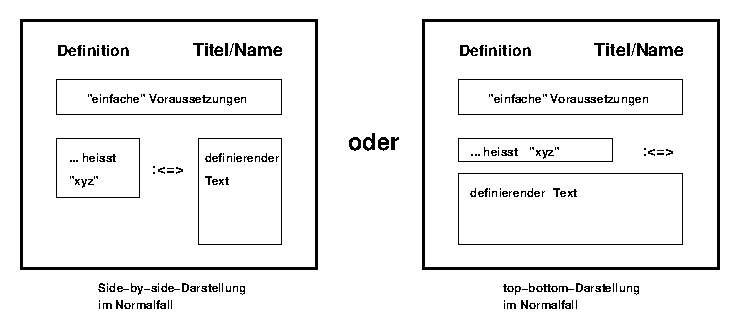
\epsfig{file=Skizzen/block_def_single_h_v.eps} 
\else
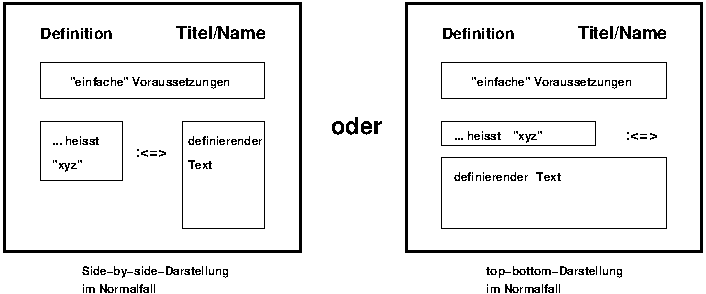
\includegraphics{Skizzen/block_def_single_h_v.pdf}
\fi
\end{center}

\textbf{Ausnahmefall Doppeldefinitionen:}

\begin{center}
\ifx\pdfoutput\undefined
   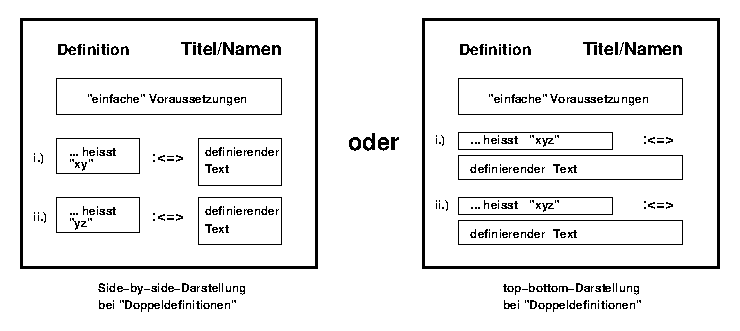
\epsfig{file=Skizzen/block_def_multi_h_v.eps} 
\else
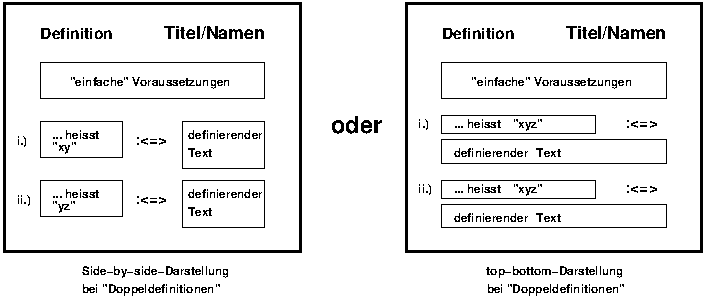
\includegraphics{Skizzen/block_def_multi_h_v.pdf} 
\fi
\end{center}

\textbf{Ausnahmefall Tripeldefinitionen} usw.: folgt entsprechend.

\vspace{5mm}

Definitionen tragen \textbf{grunds"atzlich} einen Titel; dieser
besteht i.a. aus dem Namen des zu definierenden Gegenstandes.

\clearpage

F"ur Definitionen, die sich in obiges Schema nicht einordnen lassen
(ca. 3\% !!!) steht eine Freestyle-Umgebung zur Verf"ugung, die aber
nur diese absoluten Ausnahmef"alle regelt:

\textbf{Freestyle - einfache Definition:}

\begin{center}
\ifx\pdfoutput\undefined
   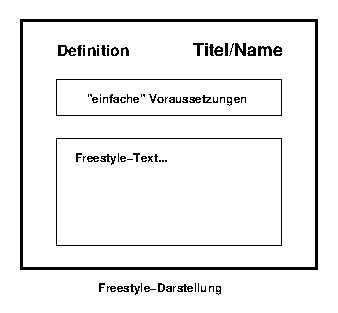
\epsfig{file=Skizzen/block_def_single_free.eps} 
\else
   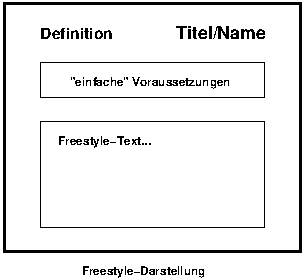
\includegraphics{Skizzen/block_def_single_free.pdf} 
\fi
\end{center}

\textbf{Freestyle - Ausnahmefall Doppeldefinitionen:}

\begin{center}
\ifx\pdfoutput\undefined
   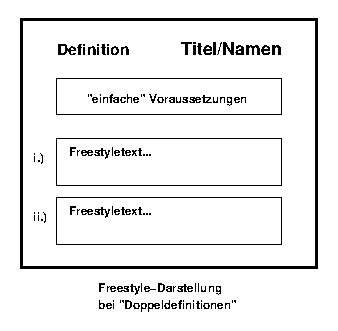
\epsfig{file=Skizzen/block_def_multi_free.eps} 
\else
   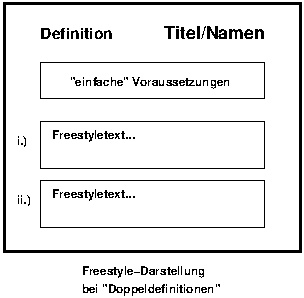
\includegraphics{Skizzen/block_def_multi_free.pdf} 
\fi
\end{center}

\textbf{Freestyle - Ausnahmefall Tripeldefinitionen} usw.: folgt entsprechend.


\clearpage



\subsubsection{Theoreme}\label{style_theoreme}

In einem Theorem wird i.a. genau \textbf{eine} Aussage vorgestellt.\\
Ausnahmen sind jedoch dann zul"assig, wenn die betreffenden Aussagen
inhaltlich so stark verkn"uft sind, da"s sie praktisch ``immer''
gemeinsam zitiert werden.

\vspace{5mm}

Die bildhaften/strukturierten Aufbauten folgen den u.s. Schemata:

\vspace{5mm}

\textbf{Der Normalfall; Implikationen und S"atze f"ur Eigenschaften:}

\begin{center}\label{block_theorem_impl_single_h_v}
\ifx\pdfoutput\undefined
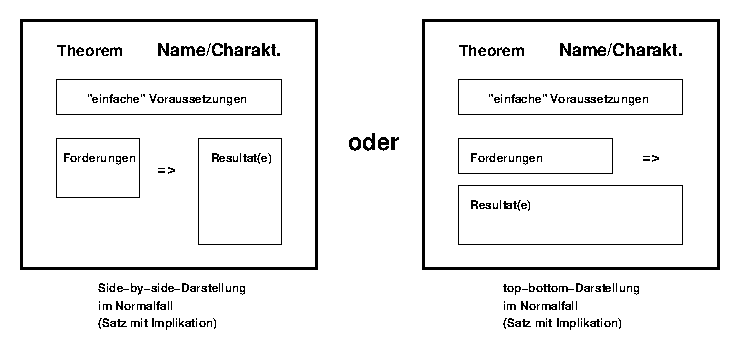
\epsfig{file=Skizzen/block_theorem_impl_single_h_v.eps} 
\else
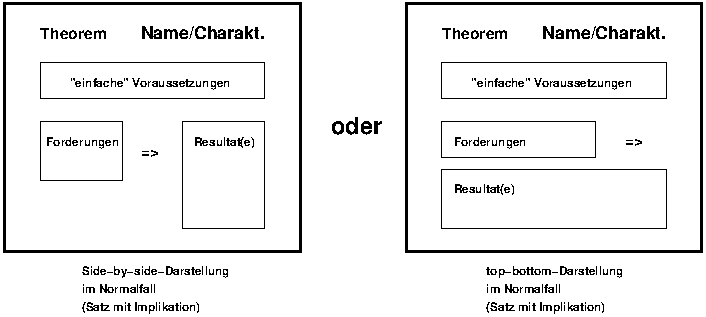
\includegraphics{Skizzen/block_theorem_impl_single_h_v.pdf} 
\fi
\end{center}

\begin{center}
\ifx\pdfoutput\undefined
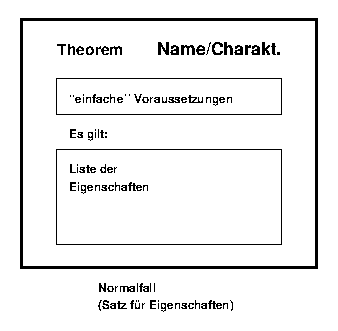
\epsfig{file=Skizzen/block_theorem_eigen_single_h_v.eps} 
\else
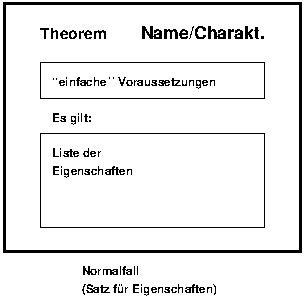
\includegraphics{Skizzen/block_theorem_eigen_single_h_v.pdf} 
\fi
\end{center}


\clearpage

\textbf{Der Normalfall; "Aquivalenzen und S"atze f"ur "aquivalente Eigenschaften:}

\begin{center}
\ifx\pdfoutput\undefined
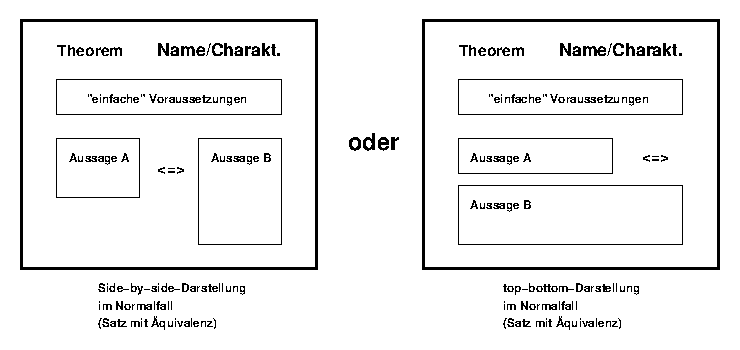
\epsfig{file=Skizzen/block_theorem_aequi_single_h_v.eps} 
\else
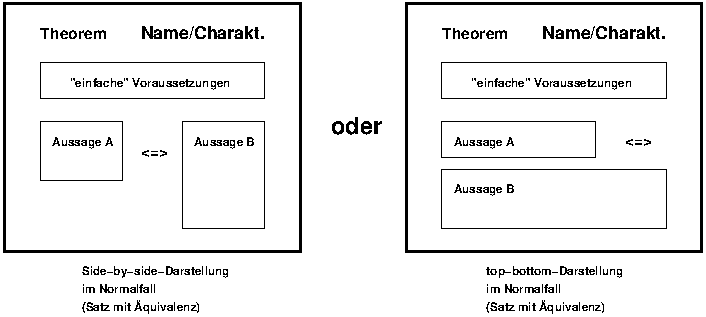
\includegraphics{Skizzen/block_theorem_aequi_single_h_v.pdf} 
\fi
\end{center}

\begin{center}
\ifx\pdfoutput\undefined
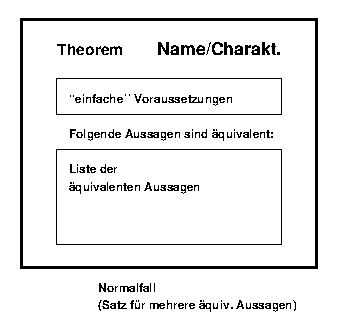
\epsfig{file=Skizzen/block_theorem_multaequi_h_v.eps} 
\else
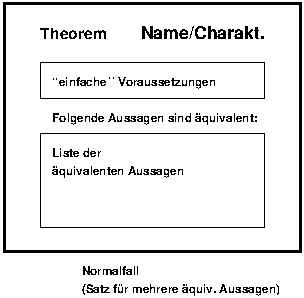
\includegraphics{Skizzen/block_theorem_multaequi_h_v.pdf} 
\fi
\end{center}

\clearpage


\textbf{Ausnahmefall Doppeltheorem; Implikationen:}

\begin{center}
\ifx\pdfoutput\undefined
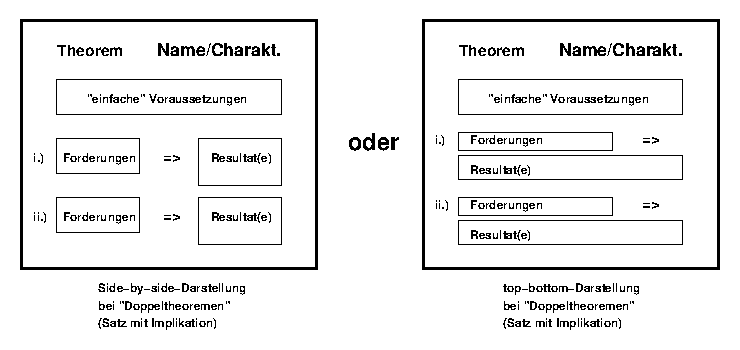
\epsfig{file=Skizzen/block_theorem_impl_multi_h_v.eps} 
\else
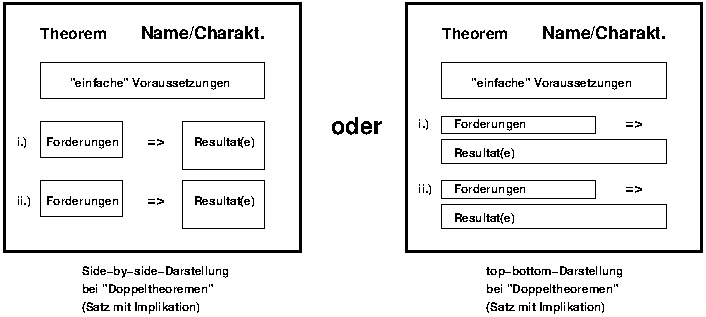
\includegraphics{Skizzen/block_theorem_impl_multi_h_v.pdf} 
\fi
\end{center}

\textbf{Ausnahmefall Doppeltheorem; "Aquivalenzen:}

\begin{center}
\ifx\pdfoutput\undefined
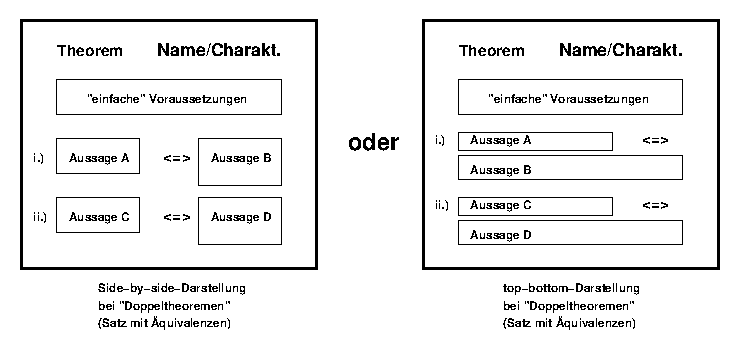
\epsfig{file=Skizzen/block_theorem_aequi_multi_h_v.eps} 
 \else
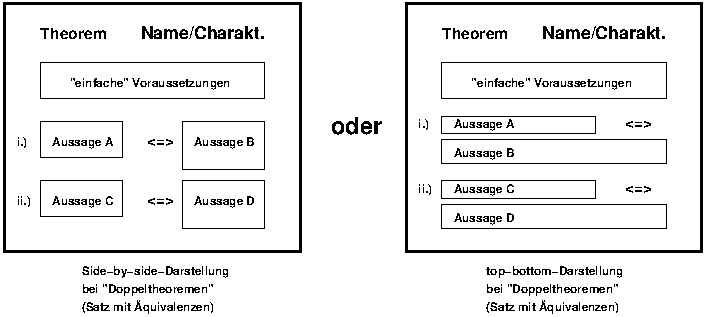
\includegraphics{Skizzen/block_theorem_aequi_multi_h_v.pdf} 
\fi
\end{center}


\textbf{Ausnahmefall Tripeltheorem} usw.: folgt entsprechend.

\vspace{5mm}

Theoreme tragen \textbf{optional} einen Titel; dieser besteht
i.a. entweder aus dem ``offiziellen Namen'' eines Satzes (etwa ``Satz
von Bolzano-Weierstra"s'') oder aus einer inhaltlichen Charakterisierung
(etwa ``Grundlegende Eigenschaften der e-Funktion'')\footnote{Es ist
offensichtlich, da"s es nicht f"ur jeden Satz pr"agnante Titel in
obigem Sinne gibt: da solche Titel aber zur Orientierung sehr
hilfreich sind, sollte diese Angabe soweit m"oglich stets erfolgen.}.

\clearpage


\subsubsection{Lemmata}

F"ur Lemmata (zu verstehen als Hilfssatz) gilt inhaltlich exakt
dasselbe wie f"ur Theoreme; es werden dieselben environments
ben"otigt, es gelten dieselben Regeln zur Namensvergabe etc.

\vspace{5mm}

Somit folgen auch die bildhaften Aufbauten den bei ``Theorem''
(s. Kap. \ref{style_theoreme}) skizzierten Schemata.%\\
%Einzige Ausnahmen: die Umgebungen ``Satz f"ur Eigenschaften'' sowie ``Satz
%f"ur mehrere "aquivalente Aussagen�� werden f"ur Lemmata nicht vorgehalten
%(``Eigenschaften'' haben keinen Hilfssatzcharakter, mehrere "aquivalente
%Aussagen sind i.a. so wichtig, da"s sie Theorem-Charakter (nicht
%Hilfssatzcharakter) haben).

\clearpage


\subsubsection{Algorithmen}

In einem Algorithmus wird genau \textbf{ein} Algorithmus/\textbf{ein} 
Rechenverfahren vorgestellt.\\
Ausnahmen sind nicht vorgesehen, zum einen aus Gr"unden einer m"oglichst
weitreichenden Modularisierung, zum anderen, weil i.a. schon ein einzelner
Algorithmus ``komplex'' und damit ``seitenf"ullend'' ist.

Die bildhaften/strukturierten Aufbauten folgen den u.s. Schemata:

\vspace{5mm}

\textbf{Algorithmus:}

\begin{center}
\ifx\pdfoutput\undefined
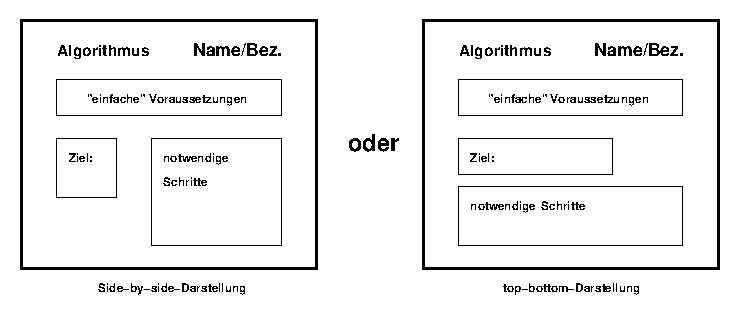
\epsfig{file=Skizzen/block_algo_single_h_v.eps} 
\else
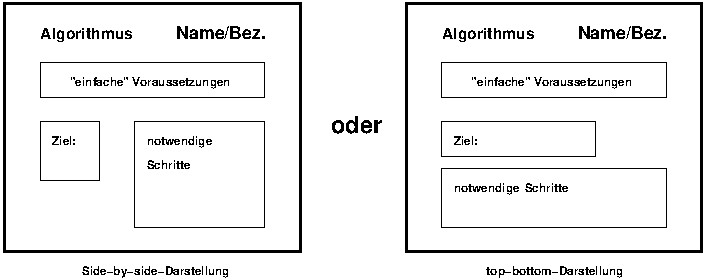
\includegraphics{Skizzen/block_algo_single_h_v.pdf} 
\fi
\end{center}


\clearpage

\subsubsection{Motivation}

\begin{list_sabina}\label{sw_motivation}
\item
\textit{kein fester} bildhafter Aufbau
\item
Ans"atze f"ur wiederkehrende Ideen bei der Gestaltung:
        \begin{sub_list_sabina}
        \item
        ``Duell'' oder Unterhaltung zweier Figuren (``Mumie'' und ihr Counterpart) 
        \item
        ...
        \end{sub_list_sabina}
\end{list_sabina}


\subsubsection{Anwendungen}

\begin{list_sabina}
\item
\textit{kein fester} bildhafter Aufbau, aber bildhafter Aufbau dennoch
angestrebt\footnote{Zum gegenw"artigen Zeitpunkt erscheint es noch zu
fr"uh, hier geeignete Umgebungen zu definieren: zun"achst m"ussten
exemplarisch einige Anwendungen auf innere Strukturen untersucht
werden.}
\end{list_sabina}


\clearpage

\subsection{Die Subelemente im einzelnen}

\subsubsection{Herleitung und Beweis}\label{block_herl_bew_struct}

Herleitungen/Beweise werden grunds"atzlich\footnote{Diese Skizze
mu"s immer erfolgen, um f"ur den Lernenden
zun"achst den Focus auf die ``zentrale Idee'', 
den ``wichtigen Beweisinput'', zu setzen.} 
zun"achst mit ihren wesentlichen Ideen skizziert;
die Skizze erfolgt listenartig.\\
Beim "Uberfahren des entsprechenden Listeneintrages k"onnen 
die zugeh"origen Details z.B. ``seitlich 
herausgefahren'' werden\footnote{Eine komplette Version, alle
Beweisteile untereinander, wird zus"atzlich angeboten.}.

Die bildhaften/strukturierten Aufbauten folgen den u.s. Schemata:

\begin{center}
\ifx\pdfoutput\undefined
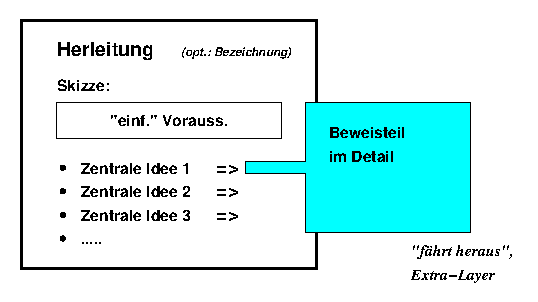
\epsfig{file=Skizzen/block_herl_struct.eps} 
\else
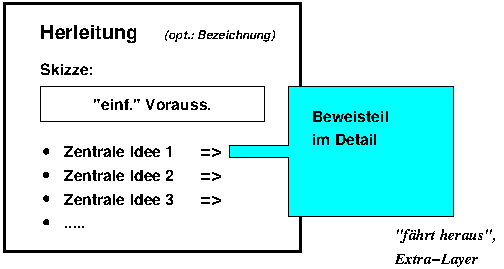
\includegraphics{Skizzen/block_herl_struct.pdf} 
\fi
\end{center}

\begin{center}\label{block_bew_struct}
\ifx\pdfoutput\undefined
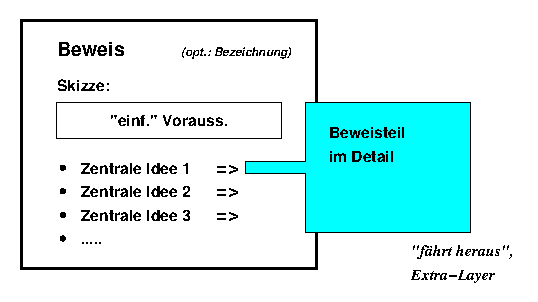
\epsfig{file=Skizzen/block_bew_struct.eps} 
\else
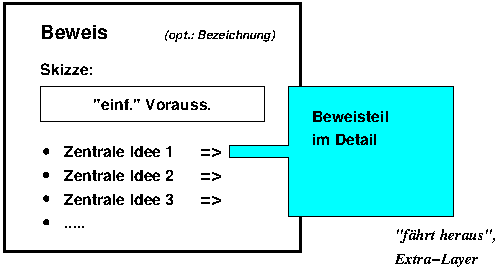
\includegraphics{Skizzen/block_bew_struct.pdf} 
\fi
\end{center}

(Die ``optionale Bezeichnung'' kann verwendet werden, wenn ein
Beweisverfahren unter einem bestimmten Namen bekannt ist oder einen
typischen mathematischen Aspekt tr"agt.)

\clearpage

\subsubsection{Historisches, Bemerkung, Motivation (zum Hauptelement)}

\textbf{Historisches} sollte wie ein wissenschaftlich-historischer
Kurzartikel verfa"st werden\footnote{Wir sind nat"urlich keine
Wissenschaftshistoriker, dennoch sollten unsere ``historischen''
Subelemente nicht so wirken, als h"atte man sie einfach aus ``Mein
kleines Geschichtslexikon'' abgeschrieben.}, ggf. angereichert durch
interaktive, multimediale und spielerische Elemente.

Das Subelement ``Historisches'' mu"s grunds"atzlich so konzeptioniert
werden, da"s es auch f"ur einen Lexikoneintrag (entweder ``alleine''
oder zusammen mit anderen Elementen/Subelementen) verwendet werden
kann.

Aktuell sind folgende ``Auspr"agungen'' dieses Subelementes vorgesehen
(hier dargestellt zusammen mit dem dazugeh"origen Teilen, aus denen das
Subelement dann bestehen soll):

\begin{enumerate}
\item
\textbf{Personen\footnote{Auch ``Gruppen mit Namen'', etwa Bourbaki, 
sind in diesen Sinne ``Personen''...} -- Biographien:}
        \begin{sub_list_sabina}
        \item
        \textbf{Abri"s:} Lebensdaten etc., allg. Daten, zentrales Wirkungsfeld, 
        Zugeh"origkeit zu (mathematischer) Schule (incl. der Lehrer), 
        Einbettung in wissenschaftliches Umfeld
        \item
        \textbf{Math./Fachl. Werk:} "Ubersicht "uber mathematisches/fachliches Gesamtwerk
        mit klar voneinander abgegrenzten einzelnen Abs"atzen;\\
        erg"anzend gibt es jeweils eine detaillierte Darstellung dieser 
        Einzelpunkte\footnotemark.
        \item
        \textbf{"Uberfachl. Bedeutung} (opt.): kulturhistorische Bedeutung, 
        gesamtgesellschaftliches Wirken, Beeinflussung des Lebensweges
        durch politische/gesellschaftliche Gegebenheiten etc.        
	         \item
	         \textbf{Bild}
	         \item
	         \textbf{Lebensdaten}: Zusammenfassung Lebensdaten
        \end{sub_list_sabina}   
\item
\textbf{Mathematische Gebiete, Zweige -- "Ubersichtsdarstellung:}
        \begin{sub_list_sabina}
        \item
        \textbf{Abri"s:} allgemeine Informationen, Daten zur Entwicklung, 
        erstes Auftreten, urspr"ungliche Fragestellung, wichtigste Namen, etc.
        \item
        \addtocounter{footnote}{-1}
        \textbf{Math. Gebiet:} "Ubersicht "uber das mathematische Gebiet
        mit klar voneinander abgegrenzten einzelnen Abs"atzen;\\
        erg"anzend gibt es jeweils eine detaillierte Darstellung dieser 
        Einzelpunkte\footnotemark.
        \item
        \textbf{"Uberfachl. Bedeutung} (opt.): historische Bedeutung, 
        gesamtgesellschaftliche Bedeutung etc.  
        \end{sub_list_sabina}\footnotetext{Die Idee folgt etwa der Darstellung von 
        ``Beweis'' oder ``Herleitung'', allerdings ist die "Ubersicht nicht
        stichwortartig, sondern in ganzen S"atzen formuliert.}   
\item
\textbf{Einzelne bedeutende Resultate\footnote{Hierzu geh"ort etwa eine historische 
Bemerkung zur Bedeutung des Fundamentalsatzes etc., ggf. mit dem entsprechenden Hinweis auf die
beteiligten Personen...}:}
        \begin{sub_list_sabina}
        \item
        \textbf{Einzelner Abschnitt:} (k"urzerer) Text zur entsprechenden Thematik, 
        erstes Auftreten, urspr"ungliche Fragestellung, 
        weiterf"uhrende Hinweise auf Namen, Gebiete etc., insbesondere zum 
        ``dort Weiterlesen''
        \end{sub_list_sabina}   

\end{enumerate}

\clearpage

Die bildhaften/strukturierten Aufbauten folgen den u.s. Schemata:

\begin{center}
\ifx\pdfoutput\undefined
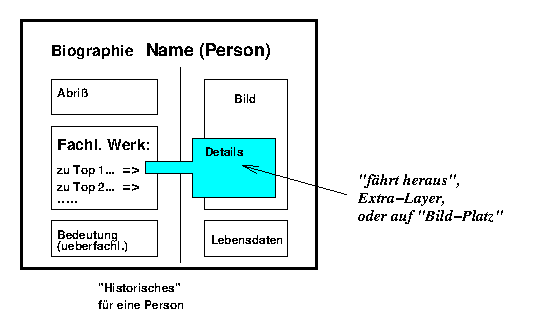
\epsfig{file=Skizzen/block_hist_person_02.eps} 
\else
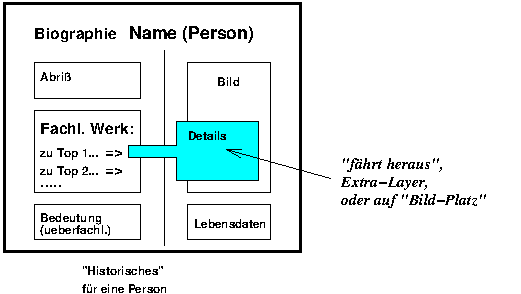
\includegraphics{Skizzen/block_hist_person_02.pdf} 
\fi
\end{center}

\begin{center}
\ifx\pdfoutput\undefined
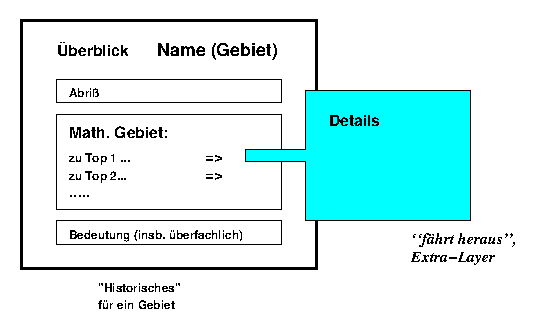
\epsfig{file=Skizzen/block_hist_gebiet.eps} 
\else
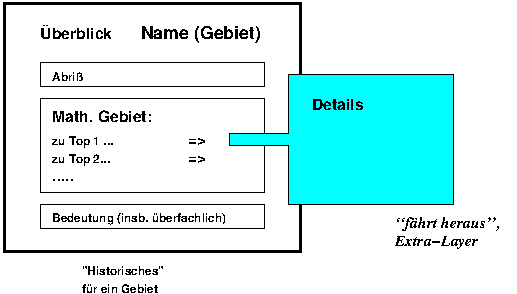
\includegraphics{Skizzen/block_hist_gebiet.pdf} 
\fi
\end{center}

\begin{center}
\ifx\pdfoutput\undefined
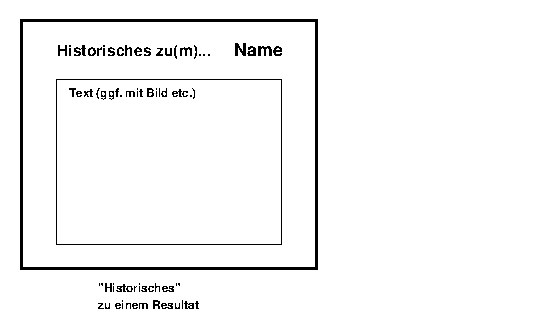
\epsfig{file=Skizzen/block_hist_resultat.eps} 
\else
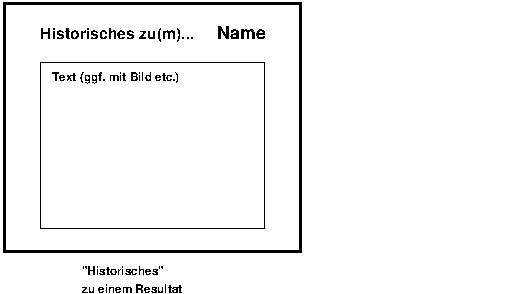
\includegraphics{Skizzen/block_hist_resultat.pdf} 
\fi
\end{center}

\clearpage

\textbf{Bemerkungen} zerfallen inhaltlich in die u.s. Gruppen.\\
Die Gruppenzugeh"origkeit wird "uber zus"atzliche selbstsprechende Icons
angezeigt\footnote{Die Gruppenzugeh"origkeit steht nicht im Vordergrund,
sollte aber einen gewissen Wiedererkennungscharkter haben.}.


\begin{enumerate}
\item
\textbf{Sloppy-Version:}
        \begin{sub_list_sabina}
        \item
        \textbf{Charakter:} ``Sloppy-Version'' des Gegenstandes des Elementes
        \item
        \textbf{Idee/Anspruch:} Kommunizieren der ``grundlegenden Idee'' 
        des Gegenstandes des Elementes 
        \item
        \textbf{Icon:} ...
        \end{sub_list_sabina}   
\item
\textbf{Direkte Bemerkung:}
        \begin{sub_list_sabina}
        \item
        \textbf{Charakter:} Achtung -- Warnung -- Merke
        \item
        \textbf{Idee/Anspruch:} agiert sehr ``direkt'' auf dem Element:
        Hinweis auf typische Fehler und Mi"sverst"andnisse, Merks"atze etc.
        \item
        \textbf{Icon:} gro"ses Ausrufezeichen 
        \end{sub_list_sabina}   
\item
\textbf{Reflektierende Bemerkung:}
        \begin{sub_list_sabina}
        \item
        \textbf{Charakter:} ``Lautes (Nach-)Denken'' "uber den Gegenstand des Elementes
        \item
        \textbf{Idee/Anspruch:} reflektiert den Gegenstand des Elementes, hinterfragt, 
        beleuchtet einzelne Aspekte...  
        \item
        \textbf{Icon:} ...
        \end{sub_list_sabina}   
\item
\textbf{Assoziative Bemerkung:}
        \begin{sub_list_sabina}
        \item
        \textbf{Charakter:} kn"upft Verbindungen zu anderen Gebieten 
        (innerhalb und au"serhalb der Mathematik)  
        \item
        \textbf{Idee/Anspruch:} geht "uber den ``Tellerrand'' hinaus
        \item
        \textbf{Icon:} ... 
        \end{sub_list_sabina}   
\end{enumerate}

Bemerkungen k"onnen grunds"atzlich ebenfalls durch ``die Mumie'' begleitet werden.\\
Insbesondere die reflektierenden Bemerkungen bieten sich hierf"ur an.


\clearpage

F"ur die \textbf{Motivation (zum Hauptelement)} gelten die gleichen
Regeln wie f"ur das Element ``Motivation''
(S. \pageref{sw_motivation}):

\begin{list_sabina}
\item
\textit{kein} fester bildhafter Aufbau
\item
Ans"atze f"ur wiederkehrende Ideen bei der Gestaltung:
        \begin{sub_list_sabina}
        \item
        F"uhrung durch ``die Mumie''
        \item
        ...
        \end{sub_list_sabina}
\end{list_sabina}


\clearpage

\subsubsection{Visualisierung, Beispiel, Tabelle}

\textbf{Beispiele} (und, mindestens genau so wichtig, Gegenbeispiele) 
haben stets eine ``sehr vollst"andige'' Version, 
in denen der Autor aber ``einfache/optionale Teile/Zwischenschritte''
als solche markiert (unsichtbares tag).
Dadurch entsteht eine ``longversion'' (f"ur den Anf"anger)
und gleichzeitig (n"amlich durch Weglassen der einfachen Zwischenschritte) 
eine komprimierte ``shortversion'' (f"ur den schon etwas versierteren Nutzer).\\
Der Benutzer kann stets die Auswahl zwischen den Versionen
treffen, auch stets ``lokal umschalten'', 
der Default richtet sich nach seinem Benutzerprofil.

Zus"atzlich werden in Beispielen alle Symbole wie
``$\Longleftrightarrow$'', ``$=$'' etc. beim "Uberfahren durch die
Maus mit einer zus"atzlichen Information versehen, die angibt, was an
der betreffenden Stelle gerade verwendet/gemacht/ausgenutzt wurde.

\vspace{5mm}

\textbf{Visualisierungen} sind i.a. interaktive definitorische oder
experimentelle Java-Applets. Solange die Applet-Factory noch nicht
steht, werden verbale Kurzbeschreibungen in den daf"ur vorgesehenen
files abgelegt, die sp"ater schnell umgesetzt werden k"onnen.

\vspace{5mm}

\textbf{Tabellen} dienen entweder f"ur vergleichende Beispiele und
Gegenbeispiele\footnote{In diesem Fall geh"oren sie strenggenommen zu
den ``Zusammenfassungselementen'', s. Fu"snote
S. \pageref{zusammenfassungselemente_footnote}.}  oder f"ur
Wertetabellen etc.\\ 
Einheitliche TeX-Styles werden definiert.





















	
\clearpage

\section{Mathematische Benennungen und Notationen}\label{benennung_notation_math_style}


\subsection{Benennungen mathematischer Begriffe}\label{benennung_style}

"Ubergeordnete Metas:

\begin{list_sabina}
\item
\textbf{``richtig'', viel Inhalt vermittelnd}
\item
\textbf{mathematischer Standard}
\end{list_sabina}


\subsubsection{Grundlagen}\label{benennung_style_grundlagen}


Es werden ausschlie"slich die u.s. Hauptvarianten im Text verwendet
(die Nebenvarianten werden im Lexikon und beim ``ersten Vorkommen'',
in der betreffenden Definition, genannt):


\begin{tabular}{!{\vrule width 1pt} >{\bfseries}m{7.5cm} | >{\itshape}m{7.5cm} !{\vrule width 1pt}}
\hline
\hline
 & \\
Hauptvariante & Nebenvariante(n)\\
& \\
\hline
\hline
bijektiv & eineindeutig \\
\hline
injektiv & eindeutig \\
\hline
surjektiv & (Abb.) auf ...\\
\hline
& ...\\
\hline
& ...\\
\hline
\hline
\end{tabular}

t.b.c.!!


\clearpage


\subsubsection{Lineare Algebra}\label{benennung_style_lina}


Es werden ausschlie"slich die u.s. Hauptvarianten im Text verwendet
(die Nebenvarianten werden im Lexikon und beim ``ersten Vorkommen'',
in der betreffenden Definition, genannt):


\begin{minipage}{\linewidth}
\renewcommand{\thefootnote}{\thempfootnote}
\begin{tabular}{!{\vrule width 1pt} >{\bfseries}m{7.5cm} | >{\itshape}m{7.5cm} !{\vrule width 1pt}}
\hline
\hline
 & \\
Hauptvariante & Nebenvariante(n)\\
 & \\
\hline
\hline
antisymmetrisch & schiefsymmetrisch\footnote{Hier bezieht sich der Begriff
  schiefsymmetrisch auf Matrizen und lineare Abbildungen.}\\
\hline
antisymmetrische Multilinearform & alternierende Multilinearform\\
\hline
Bild \newline(einer Abb. $f:V\rightarrow W$, also $f(V)$) & Wertebereich/Wertevorrat
\footnote{Die Begriffe Wertevorrat und Wertebereich sollen nicht benutzt werden, weil
  sie in der Literatur keine einheitliche Bedeutung haben und schnell zu Verwirrung f"uhren
  k"onnen.} \\
\hline
Bildbereich \newline(einer Abb. $f:V\rightarrow W$, also $W$)& Wertebereich/Wertevorrat \\
\hline
darstellende Matrix (einer lin. Abb. ) & Darstellungsmatrix, Matrixdarstellung \\ 
\hline
Defektraum \newline(einer lin. Abb. $f:V\rightarrow W$, also \newline$W\ominus f(V))$& Differenz zwischen Bildbereich und Bild\\
\hline
Dualraum\footnote{Da wir in der Linearen Algebra lediglich endlichdimensionale Lineare R"aume
  betrachten, fallen algebraischer Dualraum und topologischer Dualraum zusammen.} & dualer Raum, topol. Dualraum, topol. Dual, Dual\\
\hline
elementare Umformungen (Gau"s) & Elementarumformungen%\footnote{Der Terminus
  %``Elementarmatrizen'' soll ebenfalls nicht verwenden werden, da dieser
  %autorabh"angig einmal die beim Gaussalgorithmus ben"otigten darstellenden Matrizen der
  %elementaren Umformungen bezeichnet und andererseits die Basis des linearen Raums der
  %Matrizen.}
\\
\hline
Elementarmatrizen & elementare Matrizen\\
\hline
Kreuzprodukt & Vektorprodukt \\
\hline
Minoren  & Streichungsmatrix\\
\hline
Nullraum & Kern \\
\hline
orthogonal, -normal & rechtwinklig\\
\hline
Parallelogrammgleichung & Parallelogrammidentit"at\\
\hline
partikul"are L"osung & Partikul"arl"osung \\
\hline
Quotientenraum & Quotientenvektorraum \\
\hline
Rechte-Hand-Regel & Korkenzieherregel\\
\hline
Skalarprodukt & inneres Produkt\\
\hline
Span, span(M) & lineare H"ulle\\
\hline
Spektraldarstellung & spektrale Darstellung\\
\hline
Spur, spur(A) & Trace, tr(A)\\
\hline
Unterraum & Untervektorraum, Teilraum\\
\hline
Vektorraum & Linearer Raum\\
\hline
\hline
\end{tabular}
\end{minipage}


\subsubsection{Analysis}\label{benennung_style_ana}

t.b.c.



%======================================================================================================
\clearpage
%======================================================================================================

\subsection{Benennung mathematischer Theoreme, Algorithmen etc.}\label{theoremname_style}

"Ubergeordnete Metas:

\begin{list_sabina}
\item
\textbf{mathematischer Standard}
\item
\textbf{historisch korrekt}
\item
\textbf{(kurz)}
\end{list_sabina}

\vspace{5mm}

Bei Theoremen werden die durch ``grammatikalisches Umdrehen''
entstehende Variationen zugelassen; es kann also durchaus einmal vom
``Austauschsatz von Steinitz'', ein anderes Mal vom ``Steinitz'schen
Austauschsatz'' gesprochen werden (wenn die verschiedenen Ergebnisse
nicht gar zu grauslig klingen...).

Auch andere ``Nebenvarianten'' zugelassen, wenn dadurch keinerlei
Verwechslungsgefahren bestehen. Unten sind einige solcher F"alle
exemplarisch angedeutet, \textbf{zul"assige} Nebenvarianten sind
``italic-fett'' gekennzeichnet.


\subsubsection{Lineare Algebra}\label{theoremname_style_lina}

\begin{tabular}{| >{\bfseries}p{65mm} | >{\itshape}p{65mm} |}
\hline
\hline
 & \\
Hauptvariante & Nebenvariante(n)\\
 & \\
\hline
\hline
Austauschsatz von Steinitz & \textbf{Steinitz'scher Austauschsatz}\\
\hline
Cauchy-Schwarz'sche Ungleichung & Schwarz'sche Ungleichung\\
\hline
Gram-Schmidt'sches Orthonormierungsverfahren & Schmidt'sches Orthonormierungsverfahren \\
\hline
Laplace'scher Entwicklungssatz & \textbf{Entwicklungssatz von Laplace}\\
\hline
Satz von Jordan & \textbf{Satz von der Jordan'schen Normalform} \\
\hline
\hline
\end{tabular}

t.b.c.!!

\subsubsection{Analysis}\label{theoremname_style_ana}

\begin{tabular}{| >{\bfseries}p{65mm} | >{\itshape}p{65mm} |}
\hline
\hline
 & \\
Hauptvariante & Nebenvariante(n)\\
 & \\
\hline
\hline
Satz von Bolzano-Weierstra"s & Satz von Bolzano\\
\hline
\hline
\end{tabular}

t.b.c.!!


%======================================================================================================
\clearpage
%======================================================================================================

\subsection{Bedeutung mehrdeutiger mathematischer Begriffe}\label{benennung_mehrdeutig_style}

In diesem Abschnitt finden sich die Regelungen zur Verwendung
mathematischer Begriffe, deren Bedeutung nicht einheitlich in der
Standardliteratur verwendet wird.

\subsubsection{Lineare Algebra}

\begin{tabular}{| >{\bfseries}p{45mm} | >{\bfseries}p{40mm} | >{\itshape}p{40mm} |}
\hline
\hline
 & & \\
 & ist/sind\dots & ist/sind nicht\dots \\
 & & \\
\hline
\hline
Adjungierte (Matrix) & an 45-Grad-Achse gespiegelte Matrix & die Adjunkten \\
\hline
Elementarmatrizen & Matrizen zur Realisierung der elementaren Zeilen- und Spaltenumformungen, 
etwa beim Gau"salgorithmus & die ``kanonische Basis'' im Raum der Matrizen\\
\hline
Sesquilinearform & die math. Version (linear im 1. Eingang) & die 
physik. Version (linear im 2. Eingang)\footnote{Im entsprechenden
Modul werden beide unterschiedlichen Notationen (und ihr Hintergrund) erl"autert.}\\
\hline
$\mathbb{N}$ & Nat"urliche Zahlen incl. der Null & nicht die nat"urlichen Zahlen ohne die Null\\
\hline
\hline
\end{tabular}

t.b.c.!!

\subsubsection{Analysis}

t.b.c.!!

%======================================================================================================
\clearpage
%======================================================================================================

\subsection{Defaults zur mathematischen Pr"azision und Notation}\label{math_praezise_style}\label{notation_mathsym_style}

Folgende Metas sind zur Einigung vorgeschlagen und w"aren dann grunds"atzlich zu beachten:

\begin{list_sabina}
\item
\textbf{kurz}
\item
\textbf{mathematisch pr"azise}
\item
\textbf{``standalone'' verstehbar}\footnote{Da die einzelnen Elemente 
auch immer als Referenzen f"ur andere fachliche Kapitel dienen, kann praktisch nie
von ``Kontextwissen'' ausgegangen werden: ohne Kontextwissen kann der ``quer'' auf dieses
Element Geleitete aber nicht wissen, ob $f$ nach $\mathbb{R}$
oder $\mathbb{C}$ abbildet...}
\item
\textbf{"ubersichtlich} 
\item
\textbf{mathematischer Standard} 
\end{list_sabina}

\vspace{5mm}

\textbf{Bemerkungen:} 

\begin{enumerate}
\item
ACHTUNG: Die u.s. Angaben sind die \textit{inhaltlichen} Vorgaben an
die Pr"azision mathematischer Objekte (und \textbf{nicht} die einzigen
Darstellungen); f"ur viele der u.g. Objekte wird eine weitere Textform
(etwa ``stetig differenzierbar'' anstelle von ``$C^{1}$'')
vorgehalten.
\item
Alle mathematischen Bezeichnungen und Symbole
(Vektoren, Matrizen etc. sowie All-, Existenzquantoren usw.) werden so
programmiert, da"s mittelfristig die M"oglichkeit der
Benutzeranpassung besteht.\\
Im u.s. handelt es sich um die \textit{Default-}Einstellung, die
verbindlich verwendet wird, solange diese Anpassung an den Benutzer
noch nicht m"oglich ist, und die au"serdem als echte 
``Defaulteinstellung'' (f"ur dem System nicht bekannte User) verwendet wird.
\item
Die u.s. Formulierungen ``entscheidend'', ``relevant'' sind immer unter
den ``standalone''-Anspruch zu betrachten!\\
Kontextwissen gibt es nur \textit{innerhalb} eines Elementes, 
h"ochstens noch beim "Ubergang zu gewissen abh"angigen Subelementen.
\item
Die u.s. Regelungen beziehen sich "uberwiegend auf das Gebiet der
Linearen Algebra, die "ubrigen Regelungen m"ussen noch folgen.
\end{enumerate}



%\begin{tabular}{|l|l|p{65mm}|}
%\hline
%\hline
%\myraise{Sei} & $f \in C^{1}$ & \myraise{\footnotesize{Def.- und Werteber. nicht relevant}}\\
%\cline{2-2}
%&$f$ stetig differenzierbar & \\
%\hline
%\myraise{Sei} & $f \in C^{1} ([a,b])$ & \myraise{\footnotesize{Def.-Ber. relelvant, Werteber. nicht}}\\
%\cline{2-2}
%&$f$ stetig differenzierbar in $[a,b]$& \\
%\hline
%\myraise{Sei} & $f \in C^{1} ([a,b]), \mathbb{C})$ & \myraise{\footnotesize{Def.- und Werteber. relevant}}\\
%\cline{2-2}
%&$f$ stetig differenzierbar in $[a,b]$ nach $\mathbb{C}$& \\
%\hline
%\hline
%\end{tabular}

\clearpage
\vspace{5mm}

\textbf{Die Regelungen:} 

\begin{list_sabina}
\item
\textbf{Quantoren:} $\forall$ und $\exists$ (alte Notation)
\item
\textbf{Skalare\footnote{Skalare kommen in verschiedensten Kontexten vor 
und es haben sich vielfach bestimmte Buchstaben f"ur bestimmte Sachverhalte 
etabiliert: diesen ``Standardkonventionen soll stets so weit wie m"oglich 
gefolgt werden.}}: kleiner nicht-fetter Buchstabe, Buchstabenwahl nach 
Bedarf, griechische Buchstaben grunds"atzlich zul"assig
\item
\textbf{Vektorr"aume}:
        \begin{sub_list_sabina}
        \item
        $V$: korrekt, wenn der K"orper nicht entscheidend ist
        \item
        $V [\mathbb{C}]$: korrekt, wenn der K"orper relevant ist
        \item
        Notation/Name Vektorr"aume: $V, W$ oder $V_{1},V_{2},...,V_{n}$ 
        \item
        Notation/Name Vektoren: $\mathbf{v}, \mathbf{w}$ oder 
        $\mathbf{v_{1}},\mathbf{v_{2}},...,\mathbf{v_{n}}$ (klein und fett)
        \item
        Notation/Name Vektorr"aume mit Zusatzstruktur: einfach $V$ und
        nicht $<V, \langle \cdot, \cdot \rangle>$
        \end{sub_list_sabina}
\item
\textbf{Basen}:
        \begin{sub_list_sabina}
        \item
        allg. Basis: $\{\mathbf{b_{1}}, \mathbf{b_{2}}, ..., \mathbf{b_{n}}\}$ 
        (bzw. $\{\tilde{\mathbf{b_{1}}}, \tilde{\mathbf{b_{2}}}, ..., \tilde{\mathbf{b_{n}}}\}$, falls eine zweite ben"otigt wird)
        \item
        kanon. Basis des $\mathbb{R}^{n}$: $\{\mathbf{e_{1}}, \mathbf{e_{2}}, ..., \mathbf{e_{n}}\}$
        \end{sub_list_sabina}
\item
\textbf{Normen}:
        \begin{sub_list_sabina}
        \item
        Standardnorm: $\| \cdot \|$
        \item
        Betrag: $| \cdot |$
        \item
        allg. Norm: mit Index, wenn nicht die Standardnorm gemeint ist, z.B. 
        $\| \cdot \|_{\infty}$
        \end{sub_list_sabina}
\item
\textbf{Funktionenr"aume}:
        \begin{sub_list_sabina}
        \item
        $C^{1}$: korrekt, wenn sowohl Werte- als auch Definitionsbereich 
        nicht entscheidend sind
        \item
        $C^{1}((a,b)), C^{1}(O)$\footnote{$O\subset\mathbb{R}^n$ offen.}: korrekt, wenn der Definitionsbereich (und dessen ``Struktur'') 
        relevant ist, der Wertebereich aber nicht
        \item
        $C^{1}((a,b), \mathbb{C})$: korrekt, wenn sowohl Definitions- als 
        auch Wertebereich relevant sind
        \item
        Notation/Name Funktionenr"aume: entsprechend mathematischem Standard
        \item
        Notation/Name Funktionen: $f, g$ oder $f_{1},f_{2},...,f_{n}$ 
        \end{sub_list_sabina}
\item
\textbf{R"aume linearer Abbildungen}:
        \begin{sub_list_sabina}
        \item
        $\mathcal{L}(V,W)$: (einzige Form\footnote{Das zwar ist nicht konsistent
        mit der Festlegung f"ur allg. Funktionenr"aume, aber 
        $L \in \mathcal{L}$ sagt einfach niemand...}) 
        \item
        Notation/Name von R"aumen linearer Abbildungen: $\mathcal{L}$ oder $\mathcal{L}_{1}, \mathcal{L}_{2}, ..., \mathcal{L}_{n}$
        \item
        Notation/Name von linearen Abbildungen: $L$ oder $L_{1},L_{2},...,L_{n}$ (gro"s)
        \end{sub_list_sabina}
\item
\textbf{Matrizenr"aume}:
        \begin{sub_list_sabina}
        \item
        $\mathcal{M}$: korrekt, wenn sowohl die Dimension als auch der zugrundeliegende
        K"orper nicht relevant sind
        \item
        $\mathcal{M}(m \times n)$: korrekt, wenn die Dimension relevant ist, 
        der K"orper aber nicht
        \item
        $\mathcal{M}(m \times n, \mathbb{R})$: korrekt, wenn sowohl die Dimension als 
        auch der K"orper relevant sind
        \item
        Notation/Name von Matrizenr"aumen: s.o.
        \item
        Notation/Name von Matrizen: $\mathbf{A}, \mathbf{B}$ oder 
        $\mathbf{A}_{1},\mathbf{A}_{2},...,\mathbf{A}_{n}$ (gro"s und fett)
        \item
        Notation Einheitsmatrix: $\mathbf{E}$ (gro"s und fett)\footnote{Wenn zus"atzlich die Dimension
          gekennzeichnet werden muss, dann schreiben wir $E_{n\times n}$.}
        \end{sub_list_sabina}
\item
\textbf{Dualr"aume}:
        \begin{sub_list_sabina}
        \item
        $V^{\ast}$: Dualraum eines allg. Vektorraumes
        \item
        $(\mathbb{R}^n)^{\ast}$: Dualraum des $\mathbb{R}^n$
        \end{sub_list_sabina}
\item
\textbf{R"aume der Bilinearformen}:
        \begin{sub_list_sabina}
        \item
        $\mathbf{B}(V,W)$: einzige Form
        \item
        Notation/Name von R"aumen von Bilinearformen: s.o.
        \item
        Notation/Name einer allg. Bilinearform: ???\footnote{Vorschl"age???}% $F, G$ oder $F_{1}, F_{2}, ..., F_{n}$
        \item
        Standardskalarprodukt: $\langle \cdot, \cdot \rangle$ (eckige Klammer)
        \item
        allg. Skalarprodukt: mit Index, wenn nicht das Standardskalarprodukt gemeint ist, z.B.
        $\langle \cdot, \cdot \rangle_{L^2}$
        \item
        Pseudo-Skalarprodukt\footnote{Gemeint ist das ``Skalarprodukt'' 
        der Minkowski-Metrik. Physiker kennzeichnen das Ding h"aufig 
        "uberhaupt nicht...}:  $``\langle \cdot, \cdot \rangle$'' 
        (eckige Klammern in Anf"uhrungszeichen)
        \end{sub_list_sabina}
\item
\textbf{R"aume der Multilinearformen}:
        \begin{sub_list_sabina}
        \item
        $\mathbf{\Lambda}{(V_{1}, \dots, V_{n})}$: einzige Form
        \item
        Notation/Name von R"aumen von Multilinearformen: s.o.
        \item
        \addtocounter{footnote}{-1}
        Notation/Name einer Multilinearform: ???\footnote{Vorschl"age???}% $F, G$ oder $F_{1}, F_{2}, ..., F_{n}$
        \item
        Notation/Name von Tensoren: $T$ und weitere geeignete Buchstaben\footnote{Hier 
        verh"alt es sich "ahnlich wie bei den Skalaren: bestimmte Buchstaben werden
        f"ur bestimmte Tensoren verwendet, etwa $G$ f"ur den metrischen Tensor der
        ART usw.}, 
        kovariante Indices unten, kontravariante Indeces oben, Einsteinkonvention
        \end{sub_list_sabina}
\end{list_sabina}


t.b.c.!!






























	
\clearpage


%***************************************************************************************

\end{document}


















